\documentclass{article}
\usepackage[UTF8]{ctex}
\setmainfont{Calibri Light}
\usepackage{setspace}
\renewcommand{\baselinestretch}{1.2}
\usepackage{amsmath,bm}
\usepackage{framed} 
\usepackage{wrapfig}
\usepackage{amssymb}
\usepackage{ntheorem}
\usepackage{graphicx}
\usepackage{bbm}
\usepackage{hyperref}
\hypersetup{
	colorlinks=true,
	linkcolor=blue,
	filecolor=cyan,      
	urlcolor=red,
	citecolor=green,
}
\newtheorem{theorem}{Theorem}
\newtheorem{corollary}{Corollary}
\newtheorem{lemma}{Lemma}
\newtheorem*{proof}{Proof}
\setlength{\parindent}{2em}
\author{Siheng Zhang\\zhangsiheng@cvte.com}
\title{Chapter \textbf{\textit{4}} Linear Classification}
\date{\today}
\usepackage[a4paper,left=18mm,right=18mm,top=25mm,bottom=25mm]{geometry} 

\begin{document}
\maketitle  

This part corresponds to \textbf{Chapter 1,3,4 of PRML, Chapter of UML}, and mainly answers the following questions:

\begin{itemize}
\item 
\end{itemize}

\tableofcontents
\newpage

\section{Linear discriminant functions}
	In the last chapter, we stops at the linear classification of binary classification task,
	
	\begin{equation}
	h(\mathbf{x})=\mathbf{w}^\top \mathbf{x} + w_0 = \sum_{j=1}^d w_j x_j + w_0
	\label{eq:linear}
	\end{equation}
in which $\mathbf{w}$ is weight vector, and $w_0$ is bias. For convenience, we introduce an additional input value $x_0 = 1$ and drop the bias notation. The input vector is assigned to class $C_1$ iff. $h(\mathbf{x})\geq 0$ and to class $C_2$ otherwise.

	Consider two points $\mathbf{x}_1,\mathbf{x}_2$ on the decision boundary, i.e., $\mathbf{w}^\top (\mathbf{x}_1 - \mathbf{x}_2) = 0$, hence $\mathbf{w}$ is orthogonal to the decision boundary. And the distance from the origin to the decision boundary is $\mathbf{w}^\top \mathbf{x} / \|\mathbf{w}\|=-w_0/\|\mathbf{w}\|$.
	
	\begin{framed}
	\begin{scriptsize}
	\begin{spacing}{1.2}
	\noindent\textit{\textbf{remark1: extend to multiple classes.}  \textbf{one-versus-the-rest} For each class $k=1,2,...,K$, each classifier judge whether an example is $C_k$ or not. So there are $K$ classifiers needed;  \textbf{one-versus-one} An alternative is to introduce $\frac{K(K-1)}{2}$ binary discriminant functions, one for every pair of classes (but will lead to ambiguous region).}
	\end{spacing}
	\end{scriptsize}
	\end{framed}
		
	\subsection{VC dimension}
	The class of linear function (Eq. \ref{eq:linear}) represents a hypothesis set  \textit{half-space}, denoted as $HS_d$. Its VC dimension is $d+1$.  It follows that we can learn half-space using the ERM paradigm with a sample size of $\Omega(\frac{d+\log(1/\delta)}{\epsilon})$. 

	\begin{framed}
	\begin{scriptsize}
	\begin{spacing}{1.2}
	\noindent\textit{\textbf{remark2: proof.} Firstly, we should show that any set of $d+1$ points in $\mathcal{R}^d$ can be shattered by $HS_d$. Consider the set of vectors $\mathbf{0}, \mathbf{e}_1, ..., \mathbf{e}_d$ where for every i the vector $\mathbf{e}_i$ is the all zeros vector except 1 in the i-th entry. This set can be shattered by $HS_d$ by set $\mathbf{w}=[y_1-b,\cdots,y_d-b,b]$.}
	
	\textit{Secondly, we should show there exists a point set of $d+2$ points in $\mathcal{R}^{d}$ that cannot be shattered by half-space. Denote the points as $\mathbf{x}_1, \mathbf{x}_2, \cdots, \mathbf{x}_{d+1}, \mathbf{x}_{d+2}$. There must be some $a_i, i=1,2,\cdots,d+2$ (not all of them are zero) which satisfy that $\sum_{i=1}^{d+2} a_i \mathbf{x}_i = \mathbf{0}$. Split the $a_i$ into two sets $I={i,a_i>0}$ and $J={i,a_i<0}$, then we have }
	
	\begin{equation*}
	\sum_{i\in I} a_i \mathbf{x}_i = \sum_{i \in J} |a_i| \mathbf{x}_i
	\end{equation*}
	\textit{If the VC dimension is $d+1$, then there must be some $\mathbf{w}$ such that $\mathbf{w}^\top \mathbf{x}_i > 0, \forall i \in I$ and $\mathbf{w}^\top \mathbf{x}_i < 0, \forall i \in J$. It follows that}
	
	\begin{equation*}
	0 < \sum_{i \in I} a_i \mathbf{w}^\top \mathbf{x}_i = \mathbf{w}^\top  \sum_{i \in I} a_i \mathbf{x}_i = \mathbf{w}^\top  \sum_{i \in J} |a_i| \mathbf{x}_i =  \sum_{i \in J} |a_i| \mathbf{w}^\top \mathbf{x}_i  < 0
	\end{equation*}
	\noindent\textit{which leads to a contradiction.}
	\end{spacing}
	\end{scriptsize}
	\end{framed}
	 In the follow, we introduce different solutions to halfspaces. Except for the solutions in the chapter, we can also use a perceptron algorithm to implement ERM rule, which is left in the chapter of neural networks.
	 
\section{Linear programming}
	Linear Programming(LP) has the common form of
	\begin{equation*}
	\begin{split}
	&\min_\mathbf{w} \mathbf{u}^\top \mathbf{w} \\
	s.t. & \mathbf{Aw} \geq \mathbf{v}
	\end{split}
	\end{equation*}
	
	In the realizable (namely, separable) case, we are looking for $\text{sign}(\mathbf{w}^\top \mathbf{x}_i)=y_i$, i.e., $y_i(\mathbf{w}^\top \mathbf{x}_i)> 0, \forall i$. Define $\gamma=\min_i y_i(\mathbf{w}^\top \mathbf{x}_i)$ and let $\mathbf{w}'=\frac{\mathbf{w}}{\gamma}$, then we have $\mathbf{w}'^\top (y_i \mathbf{x}_i)\geq 1 $. With a dummy objective, it leads to LP's form.
	
\section{Least squares} 
	 
	 Least squares algorithm implements the ERM rule for the hypothesis class with respect to the squared loss. The weight vector can be determined by minimizing a sum-of-squares error function 
	$$\sum_i \|\mathbf{y}_i- \mathbf{w}^\top \mathbf{x}_i\|^2$$
	
Taking derivatives w.r.t. $\mathbf{w}$ and setting it to zero leads to

	$$\mathbf{w} = \mathbf{X}^\dagger \mathbf{Y} = (\mathbf{X}^\top \mathbf{X})^{-1} \mathbf{X}^\top \mathbf{Y}$$
in which $\mathbf{X}\in \mathcal{R}^{n\times d}$ and $\mathbf{X}^\dagger$ is the  \textit{Moore-Penrose pseudo-inverse}.
	
	Linear classification treats a problem with multiple targets to be multiple problems with single target each problem. If every target vector satisfies some  linear constraint $\mathbf{a}^\top \mathbf{y} + b = 0$, then the model prediction given by least-squares solution is $\mathbf{a}^\top h(\mathbf{x}) + b = 0$. Thus if we use a one-hot encoding for $K$ classes, the predictions made by the model will sum up to 1. However, this constraints alone is not sufficient to allow the model outputs to be interpreted as probability because they may not lie in the interval $(0,1)$.

\section{Fisher's linear discriminant}
	
	One way to view a linear classification model is in terms of \textit{dimensionality reduction}, \textit{i.e.}, projection from $\mathcal{R}^d$ to $\mathcal{R}$. By adjusting the components of the weight vector $\mathbf{w}$, we can select a projection that maximizes the class separation. To begin with, consider a two-class problem ($n_1$ points of class $C_1$ and $n_2$ points of class $C_2$), so that the mean vectors of the two classes are given by $\mathbf{m}_k = \frac{1}{n_k} \sum_{\mathbf{x}_n \in C_k} \mathbf{x}_n, k=1,2$.

	The simplest measure of the separation of the classes, when projected onto $\mathbf{w}$, is the separation of the projected class means. This suggests that we might choose $w$ so as to
	\begin{equation*}
	\max_\mathbf{w} m_2- m_1=\mathbf{w}^\top (\mathbf{m}_2-\mathbf{m}_1)
	\end{equation*}
where $m_k=\mathbf{w}^\top \mathbf{m}_k$ is the mean of the projected data from class $C_k$. 

	This expression can be made arbitrarily large simply by increasing the magnitude of $\mathbf{w}$. To solve this problem, we could constrain $\mathbf{w}$ to have unit length, i.e., $\|\mathbf{w}\|_2=1$. Using a Lagrange multiplier, it turns to maximize $\mathbf{w}^\top (\mathbf{m}_2-\mathbf{m}_1) + \lambda (\|\mathbf{w}\|_2-1)$, which leads to $\mathbf{w}\propto \mathbf{m}_2-\mathbf{m}_1$.
	
	\begin{wrapfigure}{r}{10cm}
	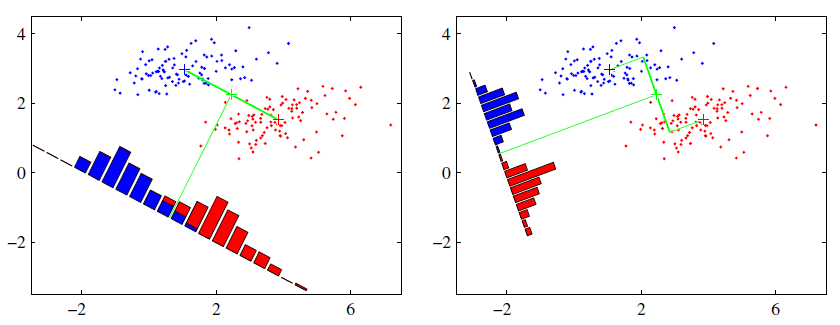
\includegraphics[scale=.7]{C4 fisher.png}	
	\label{fig4.1}
	\end{wrapfigure}
However, some outliers, which lays far from its class and close to the other class, may be mis-classified after projection, even though the dataset is linearly separable (see figure \ref{fig4.1}). This indicates that the objective above still needs to be improved. In fact, besides maximizing the separation margin, the projection is expected to reduce the inner-class variance. Denote the variance as $s_k^2=\sum_{\mathbf{x}_n\in C_k} (\mathbf{w}^\top\mathbf{x}_n-m_k)^2$, the objective is given by
	
	
	\begin{equation}
	\max_\mathbf{w} J(\mathbf{w}) = \frac{(m_2-m_1)^2}{s_1^2+s_2^2} 
	= \frac{\mathbf{w}^\top \mathbf{S}_B \mathbf{w}}{\mathbf{w}^\top \mathbf{S}_W \mathbf{w}}
	\end{equation}
in which $\mathbf{S}_B=(\mathbf{m}_2-\mathbf{m}_1)(\mathbf{m}_2-\mathbf{m}_1)^\top, \mathbf{S}_W=\sum_{k=1}^2\sum_{\mathbf{x}_n\in C_k}(\mathbf{x}_n-\mathbf{m}_k)(\mathbf{x}_n-\mathbf{m}_k)^\top$. Setting the derivative to zero leads to $(\mathbf{w}^\top \mathbf{S}_B \mathbf{w}) \mathbf{S}_W \mathbf{w} = (\mathbf{w}^\top \mathbf{S}_W \mathbf{w}) \mathbf{S}_B \mathbf{w}$. Since we just need the direction, we can neglect scalar factors. Besides,  $\mathbf{S}_B \mathbf{w}$ is always in the direction of $\mathbf{m}_2 - \mathbf{m}_1$. So the optimizer is $\mathbf{w}\propto \mathbf{S}_W^{-1} (\mathbf{m}_2-\mathbf{m}_1)$.
	
	\begin{framed}
	\begin{scriptsize}
	\begin{spacing}{1.2}
	\noindent\textit{\textbf{remark3: Isotropic.} If $\mathbf{S}_W$ is unit matrix (i.e., the data distribution of each class is isotropic), then the solution degenerates to $	\mathbf{w}\propto \mathbf{m}_2-\mathbf{m}_1$.} 

	\end{spacing}
	\end{scriptsize}
	\end{framed}
	
\subsection{Relation to least squares}

	The least-squares approach expect the \textbf{model predictions as close as possible to target values}. By contrast, the Fisher criterion was derived by \textbf{maximizing class separation in the output space}. It is interesting to see the relationship between these two approaches. In particular, we shall show that, \textbf{for the two-class problem, the Fisher criterion can be obtained as a special case of least squares}.

	Denote $n$ to be the total number of training samples, $n_1$ be the number of class 1 and $n_2$ be the number of class 2. For class 1, we take the label as $y=n/n_1$, for class 2, we take the label as $y=-n/n_2$, then we have $\sum_i y_i = n_1 * n / n_1 - n2 * n / n_2 = 0$.
	
	Here, we consider the derivatives with regard to weight and bias, \textit{i.e.}, the loss is
	
	$$\frac{1}{2}\sum_i (y_i - \mathbf{w}^\top \mathbf{x}_i - w_0)^2$$
Setting its derivatives to zero, we obtain

	\begin{equation}
	\sum_i (y_i - \mathbf{w}^\top \mathbf{x}_i - w_0) = 0
	\label{ls1}
	\end{equation}
	
	\begin{equation}
	\sum_i (y_i - \mathbf{w}^\top \mathbf{x}_i - w_0) \mathbf{x}_i= 0
	\label{ls2}
	\end{equation}
Solving the Eq.\ref{ls1} leads to 	$w_0=-\mathbf{w}^\top \mathbf{m}$, in which $\mathbf{m}$ is the mean of data. Bring it to Eq.\ref{ls2}, we obtain that

	$$
	\sum_i \mathbf{w}^\top (\mathbf{x}_i - \mathbf{m}) \mathbf{x}_i = \sum_i y_i \mathbf{x}_i 
	$$
The right-side can be written as 

	$$ 
	 \sum_i y_i \mathbf{x}_i  = \sum_{\mathbf{x}_i \in C_1} y_i \mathbf{x}_i + \sum_{\mathbf{x}_i \in C_2} y_i \mathbf{x}_i = \frac{n}{n_1} n_1 \mathbf{m}_1 - \frac{n}{n_2} n_2 \mathbf{m}_2 = n(\mathbf{m}_1 - \mathbf{m}_2)
	$$
And the left-side can be written as

	\begin{equation*}
	\begin{split}
	&\sum_i \mathbf{w}^\top (\mathbf{x}_i - \mathbf{m}) \mathbf{x}_i \\
	&=\sum_i \mathbf{w}^\top \mathbf{x}_i \mathbf{x}_i  - \mathbf{w}^\top \mathbf{m} \sum_i \mathbf{x}_i  \\
	&= \sum_{\mathbf{x}_i \in C_1}  \mathbf{w}^\top (\mathbf{x}_i - \mathbf{m}_1 + \mathbf{m}_1) (\mathbf{x}_i - \mathbf{m}_1 + \mathbf{m}_1) +  \sum_{\mathbf{x}_i \in C_2}  \mathbf{w}^\top (\mathbf{x}_i - \mathbf{m}_2 + \mathbf{m}_2) (\mathbf{x}_i - \mathbf{m}_2 + \mathbf{m}_2) - n\mathbf{w}^\top \mathbf{m} \mathbf{m}\\
	&= \sum_{\mathbf{x}_i \in C_1}  \mathbf{w}^\top (\mathbf{x}_i - \mathbf{m}_1) (\mathbf{x}_i - \mathbf{m}_1) + \sum_{\mathbf{x}_i \in C_1}  \mathbf{w}^\top  \mathbf{m}_1  \mathbf{m}_1 + \sum_{\mathbf{x}_i \in C_2}  \mathbf{w}^\top (\mathbf{x}_i - \mathbf{m}_2) (\mathbf{x}_i - \mathbf{m}_2) + \sum_{\mathbf{x}_i \in C_2}  \mathbf{w}^\top  \mathbf{m}_2  \mathbf{m}_2- n\mathbf{w}^\top \mathbf{m} \mathbf{m} \\
	&= S_W \mathbf{w} + n_1  \mathbf{m}_1  \mathbf{m}_1^\top \mathbf{w} +  n_2  \mathbf{m}_2  \mathbf{m}_2^\top \mathbf{w}- n\mathbf{m} \mathbf{m}^\top \mathbf{w}
	\end{split}
	\end{equation*}

Also note that $\mathbf{m}=\frac{n_1}{n}\mathbf{m}_1 + \frac{n_2}{n} \mathbf{m}_2$, Eq.\ref{ls2} finally leads to:

	$$(S_w + \frac{n_1 n_2}{n} S_B) \mathbf{w} = n(\mathbf{m}_1 - \mathbf{m}_2)$$
Note that $S_B \mathbf{w}$ is along the direction of $(\mathbf{m}_1 - \mathbf{m}_2)$, and neglect the magnitude again, we can obtain $\mathbf{w} \propto S_w^{-1} (\mathbf{m}_1 - \mathbf{m}_2)$. The result is same as Fisher's method and we get the bias in addition.

\subsection{For multi-class case}		
		
		
		 
\section{Probabilistic perspective}
	
	\subsection{Logistic regression}
	\label{sec-lr}
	
	\subsection{Iterative re-weighted least squares(IRLS)}
	
		 \textbf{perceptron algorithm.}
	 \textbf{surrogate loss.} In the agnostic (namely, non-separable) case, the implementation is computational hard. The most popular solution is to use surrogate loss functions but not the 0-1 loss in realizable case, which is left in \ref{sec-lr}.
	

\end{document}